\title{The Objeck Programmer's Guide}
\author{
        Randy Hollines \\
        objeck@gmail.com\\
}
\date{\today}

\documentclass[11pt]{article}

\usepackage{aliascnt}
\usepackage{hyperref}
\usepackage{MnSymbol}
\usepackage[pdftex]{graphicx}

\begin{document}

\maketitle
\thispagestyle{empty}

\vspace{\baselineskip}

\begin{abstract}
  An introduction to the Objeck programming language and it's
  features.  This article is intended to introduce programmers and
  compiler enthusiasts to the unique features and design of the Objeck
  programming language.  Unless otherwise noted, this article covers
  functionality that is included as part of release 3.1.  For
  additional information please refer to the
  \htmladdnormallink{general}{http://rosettacode.org/wiki/Category:Objeck}, 
  \htmladdnormallink{technical}{http://sourceforge.net/apps/mediawiki/objeck-lang/index.php?title=Objeck_Programming_Language}
and \htmladdnormallink{support}{http://groups.google.com/group/objeck-lang} websites.
\end{abstract}

\newpage
\tableofcontents
\newpage

\label{Introduction}
\section{Introduction}
The Objeck program language is an object-oriented computer language
with functional features.  The language was designed to be an easy to
use general purpose programming system.  The Objeck language allows
programmers to quickly create solutions by leveraging packaged class
libraries.  The syntax for the language was designed with symmetry in
mind and enforces the notion that there should one intuitive way to do
things. Features of the include:
\begin{itemize}
\item Support for object-oriented programming (all data types are
  treated as objects)
\item Functional support (higher-order functions)
\item Cross platform (support for OS X, Linux and Windows)
\item Concurrent runtime JIT support for Intel processors (x86 and x64)
\item Multi-threaded memory management (garbage collector)
\item Local optimizations and method inlining
\item Support for static libraries
\item Command line debugger
\end{itemize}

\section{Getting Started}

The Objeck distribution consists of a compiler, virtual machine,
debugger and binary inspection tool.  The compiler binary is named
\texttt{obc}, while the runtime virtual machine (VM) binary is named
\texttt{obr}.  Here is the world famous ``Hello World" program written
in the Objeck language:

\begin{verbatim}
bundle Default {
  class Hello {
    function : Main(args : String[]) ~ Nil {
      "Hello World!"->PrintLine();
    }
  }
}
\end{verbatim}

\subsection{Compiling Source}
The example below compiles the source program \texttt{hello.obs} into
the target binary file \texttt{hello.obe}.  The two output file types
that the compiler supports are executables and shared libraries.
Shared libraries are binary files that contain all of the metadata
needed by the compiler to relink them into executables.  Both executables
and shared libraries contain enough metadata to support runtime
introspection.  As a naming convention, executables must end in
\texttt{*.obe} while shared libraries must end in \texttt{*.obl}.

Below is an example of compiling the ``Hello World" program:
\begin{verbatim}
obc -src tests\hello.obs -dest hello.obe
\end{verbatim}

Here's a more advanced example of linking in two required class
libraries to an executable.
\begin{verbatim}
obc -src examples\xml_parser.obs -lib struct.obl,xml.obl -dest a.obe
\end{verbatim}

Additional compiler options are:
\begin{center}
  \begin{tabular}{| l | l |}
    \hline
    \emph{Option} & \emph{Description} \\ \hline \hline
    \texttt{-src} & path to source files, delimited by the `\texttt{,}' character \\ \hline
    \texttt{-lib} & path to library files, delimited by the `\texttt{,}'
    character\\ \hline
    \texttt{-tar} & target output \texttt{exe} for executable and \texttt{lib} for library; default is  \texttt{exe} \\ \hline
    \texttt{-opt} & optimization level \texttt{s0}--\texttt{s3} with \texttt{s3} being the most aggressive; default is \texttt{s0} \\ \hline
    \texttt{-dest} & output file name \\ \hline
    \texttt{-debug} & if set, produces debug out for use by the interactive debugger (see below) \\ \hline
  \end{tabular}
\end{center}

\subsection{Executing}
The command-line example below executes the \texttt{hello.obe}
executable. Note, for executables all required libraries are
statically linked in the target output file.  When compiling shared
libraries, other shared libraries are \underline{not} linked into the
target output library file.

\begin{verbatim}
obr hello.obe
\end{verbatim}

\section{The Basics}
Now lets introduce the core features of the Objeck programming
language.  \vspace{\baselineskip}

Let's first start with a list of keywords that exist in language.
These words are reserved for the language and may not be used as
variable, class or enum identifiers.

\begin{center}
  \begin{tabular}{ | c | c | c | c | c | }
    \hline
    \multicolumn{5}{|c|}{\emph{Keywords}} \\ \hline \hline
    and & As & Bool & break & bundle \\ \hline
    Byte & Char & class & critical & do \\ \hline
    each & else & enum & false & Float \\ \hline
    for & from & function & if & Int \\ \hline
    interface & label & method & native & New \\ \hline
    or & other & Parent & private & public \\ \hline
    return & select & static & true & TypeOf \\ \hline
    use & virtual & --- & while & xor \\ \hline
  \end{tabular}
\end{center}

In Objeck, all data types (excluding higher-order functions) are
treated as objects. Basic objects provide supports for boolean,
character, byte, integer and decimal types.  These basic objects can
be used to create more complex user defined objects.  The listing
below defines the basic objects that are supported in the language:

\begin{center}
  \begin{tabular}{| l | l |}
    \hline
    \emph{Type} & \emph{Description} \\ \hline \hline
    \texttt{Char} &  1--byte character \\ \hline
    \texttt{Char[]} &  character array \\ \hline
    \texttt{Bool} &  boolean value \\ \hline
    \texttt{Bool[]} &  boolean array \\ \hline
    \texttt{Byte} &  1--byte integer \\ \hline
    \texttt{Byte[]} &  byte array \\ \hline
    \texttt{Int} &  4--byte integer \\ \hline
    \texttt{Int[]} &  integer array \\ \hline
    \texttt{Float} &  8--byte decimal \\ \hline
    \texttt{Float[]} &  decimal array \\ \hline
    \texttt{Function} &  4--byte integer pair \\ \hline
  \end{tabular}
\end{center}

As mentioned above, basic types are objects and have associated
methods for each basic class type.  For example:

\begin{verbatim}
13->Min(3)->PrintLine();
3.89->Sin()->PrintLine();
-22->Abs()->PrintLine();
Float->Pi()->PrintLine();
\end{verbatim}

\subsection{Variable Declarations}
Variables can be declared for all of the basic types described above
and for user defined objects. Variables can be declared anywhere in a
program and are bound to traditional block scoping rules.  Variable
assignments can be made during a declaration or at any other point in
a program. Variables may be declared as local, instance or class
level scope.  Class level variables are declared using the
\texttt{static} keyword. A class that is derived from another class
may access it's parents variables if the parent class is declared in
one of the source programs.  \textit{If a class is derived from a
  class declared in a shared library then that class cannot access
  it's parents variables, unless an accessor method is provided.}
Local variables can be declared without specifying their data type,
such variables are bound to the right-hand side of their first
assignment. Three different declaration styles are shown below:

\begin{verbatim}
a : Int;
b : Int := 13;
c := 7;
\end{verbatim}

Types that are not initialized at declaration time are initialized
with the following default values:

\vspace{\baselineskip}
\begin{center}
  \begin{tabular}{| l | c |}
    \hline
    \emph{Type} & \emph{Initialization} \\ \hline \hline
    \texttt{Char} & `\textbackslash0' \\ \hline
    \texttt{Byte} & 0 \\ \hline
    \texttt{Int} & 0 \\ \hline
    \texttt{Float} & 0.0 \\ \hline
    Array & \texttt{Nil} \\ \hline
    Object & \texttt{Nil} \\ \hline
    Function & \texttt{Nil} \\ \hline
  \end{tabular}
\end{center}

\subsection{Expressions}
The Objeck language supports various type of expressions.  Some of
these expressions include mathematical, logical, arrays and method
calls.  The preceding sections describes some of the expressions
that are supported in Objeck.

\subsubsection{Mathematical and Logical Expressions}
The following code example demonstrates two ways to printing the
number \texttt{42}.  The first way invokes the \texttt{PrintLine()}
method for the literal \texttt{42}.  The second prints the product of
a variable and a literal.

\begin{verbatim}
bundle Default {
  class Test {
    function : Main() ~ Nil {
      42->PrintLine();
      eight := 8;
      (eight * 7)->PrintLine();
    }
  }
}
\end{verbatim}

The following mathematical operators are supported in the Objeck
language for integers and decimal types:
\begin{itemize}
\item addition (\texttt{+})
\item subtraction (\texttt{-})
\item multiplication (\texttt{*})
\item division (\texttt{/})
\item modulus -- (\texttt{\%} - for integer values only)
\item shift left -- (\texttt{<<} - for integer values only)
\item shift right -- (\texttt{>>} - for integer values only)
\end{itemize}

In addition the following assignment operators are supported:
\begin{itemize}
\item addition-equals (\texttt{+=})
\item subtraction-equals (\texttt{-=})
\item multiplication-equals (\texttt{*=})
\item division-equals (\texttt{/=})
\end{itemize}

The following bitwise operators are also supported for integer types:
\begin{itemize}
\item and (\texttt{and})
\item or (\texttt{or})
\item xor (\texttt{xor})
\end{itemize}

The [\texttt{*}, \texttt{/}, \texttt{\%}] operators have a higher
precedence than the [\texttt{+}, \texttt{-}] operators are naturally
enforced by the language. Operators of the same precedence are
evaluated from left-to-right.  Logical operations are of lower
precedence than mathematical operations. All logical operators are of
the same precedence and order is determined via left--to--right
evaluation.  The [\texttt{\&}, \texttt{|}] logical operators use
short-circuit logic; meaning that some expressions may not be executed
if evaluation criteria is not satisfied.

The following logical operators are supported in the Objeck language:
\begin{itemize}
\item and (\texttt{\&})
\item or (\texttt{|})
\item equal (\texttt{=})
\item not--equal (\texttt{<>})
\item less--than (\texttt{<})
\item greater--than (\texttt{>})
\item less--than--equal (\texttt{<=})
\item greater--than--equal (\texttt{>=})
\end{itemize}

\subsubsection{Arrays}
Objeck supports single and multi-dimensional arrays.  Arrays are
allocated dynamically from the system heap.  The memory that is
allocated for arrays is managed automatically by the garbage
collector.  All of the basic types described above (as well as user
defined types) can be allocated as arrays.  The code example below
shows how a two-dimensional array of type \texttt{Int} is allocated
and dereferenced.


\begin{verbatim}
array := Int->New[2,3];
array[0,2] := 13;
array[1,0] := 7;
\end{verbatim}

The size of an array can be obtained by calling the array's
\texttt{Size()} method.  The \texttt{Size()} method will return the
number of elements in a given array.  For a multi-dimensional array
the size method returns the number of elements in the first dimension.
Character array literals are allocated as \texttt{String} objects.
The \texttt{String} class provides support for advanced string operations.

\begin{verbatim}
string := "Hello World!";
string->Size()->PrintLine();
strings := ["Hello","World!"];
strings->Size()->PrintLine();
\end{verbatim}

The following example allocates an array of \texttt{Widget} objects.  An object must
implment it's \texttt{New} method if it's going to be instnatanced.

\begin{verbatim}
class Widget {
  New() {
  }
}

class MakeWidgets {
  function : Main(args : String[]) ~ Nil {
    widgets := Widget->New[1000];
    each(i : widgets) {
      widgets[i] := Widget->New();
    };
  }
}
\end{verbatim}

\subsubsection{Conditional Expressions}
There's also support for ternary conditional expressions.  For example
the following statement prints the value \texttt{false}. 

\begin{verbatim}
a := 7;
b := 13;
(((a < 13) ? 10 : 20) >  15)->PrintLine();
\end{verbatim}

\subsection{Statements}
Besides providing support for declaration statements the language has
support for conditional and control statements.  As with other
languages, control statements can be nested in order to provide finer
grain logical control. General control statements include \texttt{if}
and \texttt{select} statements. Basic looping statements include
\texttt{while}, \texttt{do/while}, \texttt{for} and \texttt{each}
loops.  Note, all statements end with the `\texttt{;}' character.

\subsubsection{If Statement}

An \texttt{if} statement is a control statement that executes an
associated block of code if it evaluates to \texttt{true}.  If the
evaluation statement does not evaluate to \texttt{true} than an
\texttt{else if} statement may be evaluated (if it exists), otherwise
an \texttt{else} statement will be executed (if it exists).  The
example below demonstrates an \texttt{if} statement.

\begin{verbatim}
value := Console->ReadLine()->ToInt();
if(value <> 3) {
  "Not equal to 3"->PrintLine();
}
else if(value < 13) {
  "Less than 13"->PrintLine();
}
else {
  "Some other number"->PrintLine();
};
\end{verbatim}

\subsubsection{Select Statement}

A \texttt{select} statement maps a value to 1 or more labels.  Labels
are associated to statement blocks.  A label may either be a literal
or an \texttt{enum} value.  Multiple labels can be mapped to the same
statement block.  Below is an example of a \texttt{select} statement.

\begin{verbatim}
select(v) {
   label Color->Red: {
      "Red"->PrintLine();
   }

   label 9:
   label 19: {
      v->PrintLine();
   }

   label 27: {
      (3 * 9)->PrintLine();
   }
};
\end{verbatim}

\subsubsection{While Statement}

A \texttt{while} statement is a control statement that will continue
to execute it's main body as long as it's conditional expression
evaluates to \texttt{true}.  When its conditional expression evaluates
to \texttt{false} than the loop body will cease to execute.

\begin{verbatim}
i := 10;
while(i > 0) {
   i->PrintLine();
   i -= 1;
}
\end{verbatim}

\subsubsection{Do/While Statement}

A \texttt{do/while} statement is a control statement that will execute
it's main body at least once and continue to execute it's main body as
long as its conditional expression evaluates to \texttt{true}.  When
it's conditional expression evaluates to \texttt{false} than the loop
body will cease to execute.

\begin{verbatim}
i := 10;
do { 
   i->PrintLine();
   i -= 1;
} 
while(i > 0);
\end{verbatim}

\subsubsection{For Statements}

The \texttt{for} statement is another common looping construct.  The
\texttt{for} loop consists of a pre-condition statement followed by an
evaluation expression and an update statement.

\begin{verbatim}
location := "East Bay"->ToCharArray();
for(i := 0; i < location->Size(); i += 1;) {
  location[i]->PrintLine();
}
\end{verbatim}

\subsubsection{Each Statements}

The \texttt{each} statement is a specialized version of a \texttt{for}
statement.  The \texttt{each} loop consists of a counter variable and
a data structure that has a \texttt{Size} method, such as arrays and
\texttt{Vector} classes.  The statement iterates thru all elements in
the data structure.

\begin{verbatim}
values := Int->New[3];
values[0] := 5;
values[1] := 1;
values[2] := 0;

each(i : values) {
  values[i]->PrintLine();
};
\end{verbatim}

\section{User Defined Types}

\subsection{Enums}
Enums are user defined enumerated types.  The main use of an
\texttt{enum} is to group a class of countable values, for example
colors, into a distinct category.  Once \texttt{enum} values have been
defined they may not be assigned or associated to a other
\texttt{enum} groups or integer classes.  The valid operations for
enums are as follows:

\begin{itemize}
\item assignment (\texttt{:=})
\item equal (\texttt{=})
\item not--equal (\texttt{<>})
\end{itemize}

In addition, enum values may be used in \texttt{select} statements as
conditional tests or labels.

\begin{verbatim}
enum Color {
   Red,
   Black,
   Green
}

enum Type := -100 {
   TYPES,
   CLASSES,
   INT,
   FLOAT
}
\end{verbatim}

\subsection{Classes}
Classes are user defined types that allow programmers to create
specialized data types.  Classes are made up of attributes (data) and
operations (methods).  Classes are used to encapsulate programming
logic and localize information.  Operations that are associated to a
class may either be at the class level or instance level.  Class
instances are created by calling an object's \texttt{New()} function.
Note, an object instance can only be created if one or more
\texttt{New()} functions have been defined.

\subsubsection{Class Inheritance}
Classes may be derived from other classes using the \texttt{from}
keyword.  Class inheritance allows classes to share common
functionality.  The Objeck language supports single class inheritance,
meaning that a derived class may only have one parent.  The language
also supports virtual classes, which assures that derived classes have
been defined for all required operations declared in the base class.
Virtual classes also allow the programmer to define non-virtual
methods that contain program behavior.  Virtual classes are
dynamically bound to implementation classes at runtime.
\begin{verbatim}
class Foo {
  @lhs : Int;

  New(lhs : Int) {
    @lhs := lhs;
  }

  method : native : AddTwo(rhs : Int) ~ Int {
    return 2 + rhs;
  }

  method : virtual : AddThree(int rhs) ~ Int;

  method : GetLhs() ~ Int {
    return lhs;
  }
}

class Bar from Foo {
  New(value : Int) {
    Parent(value);
  }

  method : native : AddThree(rhs : Int) ~ Int {
    return 3 + rhs;
  }

  function : Main() ~ Nil {
    bar : b := Bar->New(31);
    b->AddThree(9)->PrintLine();
  }
}
\end{verbatim}

\subsubsection{Class Casting and Identification}
An object that is inherited from another object may be either upcasted
or downcasted.  Object casting can be performed using the
\texttt{As()} operator.  The Object language detects upcasting and
downcastng at compile time. Upcasting requires a runtime check, while
down casting does not. If cross casting is detected then a compile
time error will be generated.

\begin{verbatim}
method : public : Compare(right : Base) ~ Int {
  if(right <> Nil) {
    if(GetClassID() = right->GetClassID()) {
      a := right->As(A);

      if(@value = a->Get()) {
        return 0;
      };
    ...	
\end{verbatim}

To determine if an object instance is of a certain class type (object
or interface) it's \texttt{TypeOf} method can be invoked.  This method will return
\texttt{true} if the instance is of the same or a derived type,
\texttt{false} otherwise.  This method can be used to check a class
instance type before casting it.

\begin{verbatim}
s := "FooBar";
t := s->TypeOf(String);
t->PrintLine();
\end{verbatim}

The class that a given object instance belongs to can found by calling
its \texttt{GetClassID} method.  This method returns an enum that is
associated with that instance's class type.  This method is generally
used to determine if two object instances are of the same or different
classes.

\subsubsection{Methods and Functions}
The Objeck language supports both methods and functions.  Functions are
public static procedures that may be executed by any class.  Methods
are operations that may be performed on an object instance.  Methods
have \texttt{public} and \texttt{private} qualifiers.  Methods that
are \texttt{private} may only be called from within the same class,
while \texttt{public} methods may be called from other classes.  Note,
methods are \texttt{private} by default. The Objeck language supports
polymorphic methods and functions, meaning that there can be multiple
methods with the same name within the same class as long as their
declaration arguments vary.

Methods and functions can either be executed in an interpreted or JIT
compiled mode. Interpreted execution mimics microprocessor functions
in a platform independent manner. JIT execution takes the compiled
stack code an produces native machine code. Note, that there is
initial overhead involved in the JIT compilation process since it
occurs at runtime. In addition, some methods can not be compiled into
native machine code but this is a rare case.  The keyword
\texttt{native} is used to JIT compile methods and functions at
runtime.

A function or method may be defined as \texttt{virtual} meaning that
any class that originates from that class must implement all of the
class's \texttt{virtual} methods or functions.  \texttt{Virtual}
methods are a way to ensure that certain operations are available to a
family of classes. If a class declares a \texttt{virtual} method then
the class become \texttt{virtual}, meaning that it cannot be directly
instantiated.

Below is an example of declaring a virtual method:
\begin{verbatim}
method : virtual : public : GetMake() ~ String;
\end{verbatim}

\subsection{Interfaces}
As a modern object-oriented language, Objeck supports interfaces.
Interfaces define virtual methods that must be implemented by a given
class.  A class may implement one or more interfaces.  Interface
references may be passed, dereferenced and casted in a similar manner to class
references.  Below is an example of an interface definition:

\begin{verbatim}
interface Color {
  method : virtual : public : GetColor() ~ String;
}

interface Vehicle {
  method : virtual : SetName(name : String) ~ Nil;
  method : virtual : public : GetNumberOfWheels() ~ Int;
}

class Ufo implements Vehicle, Color {
  method : public : GetColor() ~ String {
    ...
  }
  method : SetName(name : String) ~ Nil {
    ...
  }
  method : public : GetNumberOfWheels() ~ Int {
    ...
  }
}
\end{verbatim}

\subsection{Higher-Order Functions}
The Objeck language supports the notion of higher-order functions such
that a given function may be bound to a variable at runtime.
Variables are assigned based upon functional prototypes.  Prototypes
enforce strong type checking by ensuring that a function parameters
and return type are consistent between assignments.  Once a variable
is bound, it may be assigned to other variables, passed to other
functions/methods, returned from other functions/method or dynamically
evoked.  Please note, methods are not treated as higher-order
constructs only functions.

\subsubsection{Assigning and Passing Functions}
The following example shows how a function is defined and assigned to
a variable:
\begin{verbatim}
class Foo {
  function : GetSize(s : String) ~ Int {
      return s->Size();
  }
}
....
s1 : (String) ~ Int := Foo-> GetSize(String) ~ Int;
s2 := Foo->GetSize(String) ~ Int;
size1 := EnvokeSize("Hello", s1);
size2 := EnvokeSize("Hello", s2);
\end{verbatim}

\subsubsection{Envoking Functions}
The following example shows two ways that a function variable can be
assigned and envoked:
\begin{verbatim}
...
method : public : EnvokeSize(s : String, f : (String) ~ Int) ~ Int {
  return f(s);
}
...
\end{verbatim}

\section{Native Shared Library Support}
The Objeck Language has the ability to interact with native C/C++
shared libraries (shared libraries/DLLs) via runtime 
extensions.  The APIs allow a programmer to load a shared libraries and invoke native C
functions.  Data is passed between the two layers via
\texttt{Object[]}.  Basic objects such as \texttt{Int} and
\texttt{Float} types must be wrapped in \texttt{IntHolder} and
\texttt{FloatHolder} classes respectively.  Please refer to the
examples in the source code distribution for additional information.

A native function signature looks likes like the following:
\begin{verbatim}
#ifdef _WIN32
  __declspec(dllexport)
#endif
  void odbc_connect(VMContext& context);
\end{verbatim}

The \texttt{VMContext} structure contains pointers to the calculation
stack as well as utility functions that allow programmers to 
allocate VM objects and arrays.  In addition, this structure provides the
ability to invoke VM functions and methods..  

\begin{verbatim}
struct VMContext {
  long* data_array;
  long* op_stack;
  long* stack_pos;
  APITools_AllocateArray_Ptr alloc_array;
  APITools_AllocateObject_Ptr alloc_obj;
  APITools_MethodCall_Ptr call_method_by_name;
  APITools_MethodCallId_Ptr call_method_by_id;
};
\end{verbatim}

The \texttt{lib\_api.h} header file also includes helper functions
that allow programmers to access and set data that passed into the
native C function.  The following functions are available: 

\begin{itemize}
\item \begin{verbatim}APITools_GetFunctionValue\end{verbatim}
\item \begin{verbatim}APITools_SetFunctionValue\end{verbatim}
\item \begin{verbatim}APITools_GetIntValue\end{verbatim}
\item \begin{verbatim}APITools_GetIntAddress\end{verbatim}
\item \begin{verbatim}APITools_SetIntValue\end{verbatim}
\item \begin{verbatim}APITools_GetFloatValue\end{verbatim}
\item \begin{verbatim}APITools_GetFloatAddress\end{verbatim}
\item \begin{verbatim}APITools_GetStringValue\end{verbatim}
\item \begin{verbatim}APITools_SetStringValue\end{verbatim}
\item \begin{verbatim}APITools_CallMethod\end{verbatim}
\item \begin{verbatim}APITools_PushInt\end{verbatim}
\item \begin{verbatim}APITools_PushFloat\end{verbatim}
\item \begin{verbatim}APITools_GetArraySize\end{verbatim}
\item \begin{verbatim}APITools_SetIntArrayElement\end{verbatim}
\item \begin{verbatim}APITools_GetFloatArrayElement\end{verbatim}
\item \begin{verbatim}APITools_SetFloatArrayElement\end{verbatim}
\end{itemize}

\section{Debugger}
The Objeck compiler toolset contains a simple interactive read-only
debugger, which allows programmers to inspect values within their
programs.  The debugger allows programmers to set breakpoints within
methods based upon source line numbers.  The debugger can also
calculate simple arithmetic expressions involving variables and
constants. The following commands are currently supported:

\subsection{Starting the Debugger}
The source program must be compiled with the \texttt{-debug} set. The
command line debugger is started up running the \texttt{odb}
executable. The \texttt{-exe} option must be present and specify the
path to the executable.  The The \texttt{-src} option is optional and
specifies the path to the program source.  Also note, to print
instance level variables the path must start with
\texttt{@self$\rightarrow$}.

\subsection{Debugging Commands}
\begin{center}
  \begin{tabular}{| l |p{4 cm} |p{4 cm} |}
    \hline
    \emph{Command} & \emph{Description} & \emph{Example} \\ \hline \hline
    \texttt{[b]reak} &  sets a breakpoint & \texttt{b \newline b hello.obs:10} \\ \hline
    \texttt{breaks} &  shows all breakpoints &  \\ \hline
    \texttt{[d]elete} &  deletes a breakpoint & \texttt{d hello.obs:10} \\ \hline
    \texttt{clear} &  clears all breakpoints &  \\ \hline
    \texttt{[n]ext} &  moves to the next line within the same
    method/function with debug information & \\ \hline
    \texttt{[s]tep} &  moves to the next line with debug information &  \\ \hline
    \texttt{[j]ump} &  jumps out of an existing method/function and moves to the next line with debug information &  \\ \hline
    \texttt{args} &  specifies program arguments & \texttt{args "Hello World"} \\ \hline
    \texttt{[r]un} &  runs a loaded program &  \\ \hline
    \texttt{[p]rint} &  prints the value of an expression, along with
    metadata & \texttt{p locl\_value \newline p @self$\rightarrow$inst\_value} \\ \hline
    \texttt{[l]ist} &  lists a range of lines in a source file or the
    lines near the current breakpoint & \texttt{l \newline l hello.obs:10} \\ \hline
    \texttt{[i]nfo} &  displays the variables for a class & \texttt{i
      \newline i class=Foo} \\ \hline
    \texttt{stack} &  displays the method/function call stack &  \\ \hline
    \texttt{exe} &  loads a new executable & \texttt{exe "./../test.obe"} \\ \hline
    \texttt{src} &  specifies a new source path & \texttt{src "../../"} \\ \hline
    \texttt{[q]uit} &  exits a given debugging session &  \\ \hline
  \end{tabular}
\end{center}

\section{Class Libraries}
Objeck includes class libraries that provides access to system
resources, such as files and sockets, while also providing support for
basic data structures like lists and vectors.  As new class libraries
are added they will be documented in this section.

\subsection{Core}
Class support for basic datatypes.

\subsubsection{Base}
Base class for all objects.
\begin{itemize}
\item \texttt{GetClass} - returns metadata about a class
  \begin{itemize}
  \item method : public : GetClass() \textasciitilde Class
  \end{itemize}
\item \texttt{GetClassID} - returns the class ID
  \begin{itemize}
  \item method : public : native : GetClassID() \textasciitilde ClassID
  \end{itemize}
\item \texttt{GetInstanceID} - returns a unique instance ID
  \begin{itemize}
  \item method : public : native : GetInstanceID() \textasciitilde Int
  \end{itemize}
\end{itemize}

\subsubsection{Bool}
\begin{itemize}
\item \texttt{Print} - prints the current value
  \begin{itemize}
  \item method : native : Print() \textasciitilde Nil
  \end{itemize}
\item \texttt{PrintLine} - prints the current value along with a line
  return
  \begin{itemize}
  \item method : native : PrintLine() \textasciitilde Nil
  \end{itemize}
\item \texttt{ToString} - converts the current value to a
  \texttt{String} object instance
  \begin{itemize}
  \item method : native : ToString() \textasciitilde String
  \end{itemize}
\end{itemize}

\subsubsection{Char}
\begin{itemize}
\item \texttt{ToUpper} - coverts a character to a uppercase
  character
  \begin{itemize}
  \item method : public : native : ToUpper() \textasciitilde Char
  \end{itemize}
\item \texttt{ToLower} - coverts a character to a lowercase
  character
  \begin{itemize}
  \item method : public : native : ToLower() \textasciitilde Char
  \end{itemize}
\item \texttt{IsDigit} - determines if the character is a digit (in
  the range of \texttt{0-9})
  \begin{itemize}
  \item method : native : IsDigit() \textasciitilde Bool
  \end{itemize}
\item \texttt{IsChar} - determines if the character is a alpha (in the
  range of \texttt{A-Z} or \texttt{a-z})
  \begin{itemize}
  \item method : native : IsChar() \textasciitilde Bool
  \end{itemize}
\item \texttt{Min} - returns the smallest of the two numbers; returns
  the same number if they are equal
  \begin{itemize}
  \item method : native : Min(r : Char) \textasciitilde Char
  \end{itemize}
\item \texttt{Max} - returns the largest of the two numbers; returns
  the same number if they are equal
  \begin{itemize}
  \item method : native : Max(r : Char) \textasciitilde Char
  \end{itemize}
\item \texttt{Print} - prints the current value
  \begin{itemize}
  \item method : native : Print() \textasciitilde Nil
  \end{itemize}
\item \texttt{PrintLine} - prints the current value along with a line
  return
  \begin{itemize}
  \item method : native : PrintLine() \textasciitilde Nil
  \end{itemize}
\item \texttt{ToString} - converts the current value to a
  \texttt{String} object instance
  \begin{itemize}
  \item method : native : ToString() \textasciitilde String
  \end{itemize}
\end{itemize}

\subsubsection{Byte/Int}
\begin{itemize}
\item \texttt{Min} - returns the smallest of the two numbers; returns
  the same number if they are equal
  \begin{itemize}
  \item method : native : Min(r : Byte) \textasciitilde Byte
  \end{itemize}
\item \texttt{Max} - returns the largest of the two numbers; returns
  the same number if they are equal
  \begin{itemize}
  \item method : native : Max(r : Byte) \textasciitilde Byte
  \end{itemize}
\item \texttt{Abs} - returns the absolute value of the current number
  \begin{itemize}
  \item method : native : Abs() \textasciitilde Byte
  \end{itemize}
\item \texttt{Print} - prints the current value
  \begin{itemize}
  \item method : native : Print() \textasciitilde Nil
  \end{itemize}
\item \texttt{PrintLine} - prints the current value along with a line
  return
  \begin{itemize}
  \item method : native : PrintLine() \textasciitilde Nil
  \end{itemize}
\item \texttt{ToString} - converts the current value to a
  \texttt{String} object instance
  \begin{itemize}
  \item method : native : ToString() \textasciitilde String
  \end{itemize}
\end{itemize}

\subsubsection{Float}
\begin{itemize}
\item \texttt{Min} - returns the smallest of the two numbers; returns
  the same number if they are equal
  \begin{itemize}
  \item method : native : Min(r : Byte) \textasciitilde Float
  \end{itemize}
\item \texttt{Max} - returns the largest of the two numbers; returns
  the same number if they are equal
  \begin{itemize}
  \item method : native : Max(r : Byte) \textasciitilde Float
  \end{itemize}
\item \texttt{Abs} - returns the absolute value of the current number
  \begin{itemize}
  \item method : native : Abs() \textasciitilde Float
  \end{itemize}
\item \texttt{Floor} - returns the floor of the current number
  \begin{itemize}
  \item method : Floor() \textasciitilde Float
  \end{itemize}
\item \texttt{Ceiling} - returns the ceiling of the current number
  \begin{itemize}
  \item method : Ceiling() \textasciitilde Float
  \end{itemize}
\item \texttt{Sin} - returns the sine of the radian value
  \begin{itemize}
  \item method : Sin() \textasciitilde Float
  \end{itemize}
\item \texttt{Cos} - returns the cosine of the radian value
  \begin{itemize}
  \item method : Cos() \textasciitilde Float
  \end{itemize}
\item \texttt{Tan} - returns the tangent of the radian value
  \begin{itemize}
  \item method : Tan() \textasciitilde Float
  \end{itemize}
\item \texttt{ArcSin} - returns the arc sine of the radian value
  \begin{itemize}
  \item method : ArcSin() \textasciitilde Float
  \end{itemize}
\item \texttt{ArcCos} - returns the arc cosine of the radian value
  \begin{itemize}
  \item method : ArcCos() \textasciitilde Float
  \end{itemize}
\item \texttt{ArcTan} - returns the arc tangent of the radian value
  \begin{itemize}
  \item method : ArcTan() \textasciitilde Float
  \end{itemize}
\item \texttt{ToRadians} - converts degrees to radians
   \begin{itemize}
  \item method : ToRadians() \textasciitilde Float
  \end{itemize}
\item \texttt{Log} - returns the natural log of the radian value
  \begin{itemize}
  \item method : Log() \textasciitilde Float
  \end{itemize}
\item \texttt{Pi} - returns the value of Pi
  \begin{itemize}
  \item function : Pi() \textasciitilde Float
  \end{itemize}
\item \texttt{Power} - returns the exponential power value
  \begin{itemize}
  \item method : Power() \textasciitilde Float
  \end{itemize}
\item \texttt{SquareRoot} - returns the square root
  \begin{itemize}
  \item method : SquareRoot() \textasciitilde Float
  \end{itemize}
\item \texttt{Random} - returns a puedo-random number between 0.0 and
  1.0
  \begin{itemize}
  \item function : Random() \textasciitilde Float
  \end{itemize}
\item \texttt{Print} - prints the current value
  \begin{itemize}
  \item method : native : Print() \textasciitilde Nil
  \end{itemize}
\item \texttt{PrintLine} - prints the current value along with a line
  return
  \begin{itemize}
  \item method : native : PrintLine() \textasciitilde Nil
  \end{itemize}
\item \texttt{ToString} - converts the current value to a
  \texttt{String} object instance
  \begin{itemize}
  \item method : native : ToString() \textasciitilde String
  \end{itemize}
\end{itemize}

\subsubsection{String}
\begin{itemize}
\item \texttt{New}
  \begin{itemize}
  \item New()
  \item New(s : String)
  \item New(a : Char[])
  \item New(a : Byte[])
  \end{itemize}
\item \texttt{Append} - Appends a \texttt{String}, \texttt{Char[]},
  \texttt{Char}, \texttt{Int} or \texttt{Float} to the current String
  instance
  \begin{itemize}
  \item method : public : native : Append(s : String) \textasciitilde Nil
  \item method : public : native : Append(c : Char) \textasciitilde Nil
  \item method : public : native : Append(b : Byte) \textasciitilde Nil
  \item method : public : native : Append(i : Int) \textasciitilde Nil
  \item method : public : native : Append(f : Float) \textasciitilde Nil
  \item method : public : native : Append(a : Char[]) \textasciitilde Nil
  \end{itemize}
\item \texttt{Find} - returns the index of the first occurrence of a
  given Character; -1 if not found
  \begin{itemize}
  \item method : public : native : Find(c : Char) \textasciitilde Int
  \end{itemize}
  \texttt{Find} - returns the index of the first occurrence of a given
  Character; -1 if not found
  \begin{itemize}
  \item method : public : native : Find(offset : Int, c : Char) \textasciitilde Int
  \end{itemize}
\item \texttt{Find} - returns the index of the first occurrence of a
  given String; -1 if not found
  \begin{itemize}
  \item method : public : native : Find(s : String) \textasciitilde Int
  \item method : public : native : Find(s : String, offfset : Int) \textasciitilde Int
  \end{itemize}
\item \texttt{Replace} - find and replace a single string instance.
  \begin{itemize}
  \item method : public : native : Replace(find : String, replace : String) \textasciitilde String
  \end{itemize}  
\item \texttt{ReplaceAll} - find and replace all string instances.
  \begin{itemize}  
  \item method : public : native : ReplaceAll(find : String, replace : String) \textasciitilde String
  \end{itemize}
\item \texttt{Size} - returns the size of the String
  \begin{itemize}
  \item method : public : native : Size() \textasciitilde Int
  \end{itemize}
\item \texttt{IsEmpty} - returns true if the string is empty, false
  otherwise
  \begin{itemize}
  \item method : public : native : IsEmpty() \textasciitilde Bool
  \end{itemize}
\item \texttt{Get} - returns the Character at the given index or -1 if
  not found
  \begin{itemize}
  \item method : public : native : Get(i : Int) \textasciitilde Char
  \end{itemize}
\item \texttt{ToCharArray} - converts a string to a \texttt{Char[]}
  \begin{itemize}
  \item method : public : native : ToCharArray() \textasciitilde Char[]
  \end{itemize}
\item \texttt{ToInt} - converts a string to a \texttt{Int}
  \begin{itemize}
  \item method : public : native : ToInt() \textasciitilde Int
  \end{itemize}
\item \texttt{ToFloat} - converts a string to a \texttt{Float}
  \begin{itemize}
  \item method : public : native : ToFloat() \textasciitilde Int
  \end{itemize}
\item \texttt{SubString} - creates a new string that contains a subset
  of the string's contents
  \begin{itemize}
  \item method : public : native : SubString(offset : Int) \textasciitilde String
  \item method : public : native : SubString(offset : Int, length :
    Int) \textasciitilde String
  \end{itemize}
\item \texttt{Trim} - removes all leading and trailing whitespace
  \begin{itemize}
  \item method : public : native : Trim() \textasciitilde String
  \end{itemize}
\item \texttt{Pop} - removes the last character from a string 
  \begin{itemize}
  \item method : public : native : Pop() \textasciitilde Char
  \end{itemize}
\item \texttt{StartsWith} - returns true if \texttt{String} starts
  with matching pattern; returns false otherwise
  \begin{itemize}
  \item method : public : native : StartsWith() \textasciitilde Bool
  \end{itemize}
\item \texttt{EndsWith} - returns true if \texttt{String} ends with
  matching pattern; returns false otherwise
  \begin{itemize}
  \item method : public : native : EndsWith() \textasciitilde Bool
  \end{itemize}
\item \texttt{ToUpper} - coverts all lowercase characters to uppercase
  characters
  \begin{itemize}
  \item method : public : native : ToUpper() \textasciitilde String
  \end{itemize}
\item \texttt{ToLower} - coverts all uppercase characters to lowercase
  characters
  \begin{itemize}
  \item method : public : native : ToLower() \textasciitilde String
  \end{itemize}
\item \texttt{Reverse} - returns a string with reversed characters
  \begin{itemize}
  \item method : public : native : Reverse() \textasciitilde String
  \end{itemize}
\item \texttt{Equals} - compares two string returns \texttt{true} if
  they are equal
  \begin{itemize}
  \item method : public : Equals(rhs : String) \textasciitilde Bool
  \end{itemize}
\item \texttt{Compare} - compares two string returns 0 if they are
  equal
  \begin{itemize}
  \item method : public : native : Compare(rhs : Compare) \textasciitilde Int
  \end{itemize}
\item \texttt{Split} - breaks a string into tokens based upon a given
  delimiter
  \begin{itemize}
  \item method : public : native : Split(delim : String) \textasciitilde String[]
  \end{itemize}
\item \texttt{Print} - prints the current value
  \begin{itemize}
  \item method : native : Print() \textasciitilde Nil
  \end{itemize}
\item \texttt{PrintLine} - prints the current value along with a line
  return
  \begin{itemize}
  \item method : native : PrintLine() \textasciitilde Nil
  \end{itemize}
\end{itemize}

\subsubsection{Bool}
\begin{itemize}
\item \texttt{Print} - prints the current value
  \begin{itemize}
  \item method : native : Print() \textasciitilde Nil
  \end{itemize}
\item \texttt{PrintLine} - prints the current value along with a line
  return
  \begin{itemize}
  \item method : native : PrintLine() \textasciitilde Nil
  \end{itemize}
\item \texttt{ToString} - converts the current value to a
  \texttt{String} object instance
  \begin{itemize}
  \item method : native : ToString() \textasciitilde String
  \end{itemize}
\end{itemize}
 
\subsection{Data Structures}
Provides support for basic data structures such as vectors, lists,
hashes, maps, etc.  These classes are located in the `Struct'
bundle.

\subsubsection{Compare}
Interface for all objects that use comparative algorithms.
\begin{itemize}
\item \texttt{Compare} - compares two object instances; 0 if equal,
  less-then 0 if less and greater-then 0 if greater.
  \begin{itemize}
  \item method : virtual : public : Compare(rhs : System.Compare) \textasciitilde Int
  \end{itemize}
\item \texttt{HashID} - returns a unique value for the given class
  type
  \begin{itemize}
  \item method : virtual : public : HashID() \textasciitilde Int
  \end{itemize}
\end{itemize}

\subsubsection{BasicCompare}
Basic implementation of \texttt{Compare} methods.
\begin{itemize}
\item \texttt{Compare} - returns true if argument is the same
  instance, false otherwise.
  \begin{itemize}
  \item method : public : Compare(rhs : System.Compare) \textasciitilde Int
  \end{itemize}
\item \texttt{HashID} - hash value based upon instance ID
  \begin{itemize}
  \item method : public : HashID() \textasciitilde Int
  \end{itemize}
\end{itemize}

\subsubsection{List/IntList/FloatList}
The List class allow values to be added, removed and deleted from a
list.  There are two specialized version of this class:
\texttt{IntList} and \texttt{FloatList}.  The \texttt{IntList} and
\texttt{FloatList} classes use \texttt{Int} and \texttt{Float} types
respectively instead of \texttt{Compare} type.  The general class
supports the following operations:
\begin{itemize}
\item \texttt{AddBack} - adds a new value to the back of the list
  \begin{itemize}
  \item method : public : native : AddBack(value : Compare) \textasciitilde Nil
  \end{itemize}
\item \texttt{RemoveBack} - removes the last element in the list
  \begin{itemize}
  \item method : public : RemoveBack() \textasciitilde Nil
  \end{itemize}
\item \texttt{AddFront} - adds a new value to the front of the list
  \begin{itemize}
  \item method : public : native : AddFront(value : Compare) \textasciitilde Nil
  \end{itemize}
\item \texttt{RemoveFront} - removes the first element in the list
  \begin{itemize}
  \item method : public : RemoveFront() \textasciitilde Nil
  \end{itemize}
\item \texttt{Find} - finds an element in the list
  \begin{itemize}
  \item method : public : Find(value : Compare) \textasciitilde Bool
  \end{itemize}
\item \texttt{Has} - returns true if item is in list
  \begin{itemize}
  \item method : public : Has(value : Compare) \textasciitilde Bool
  \end{itemize}
\item \texttt{Insert} - inserts a new value in the position pointed to
  the cursor
  \begin{itemize}
  \item method : public : Insert(value : Compare) \textasciitilde Bool
  \end{itemize}
\item \texttt{Remove} - removes the last element in the list
  \begin{itemize}
  \item method : public : Remove() \textasciitilde Nil
  \end{itemize}
\item \texttt{Insert} - inserts an element into the current cursor
  position
  \begin{itemize}
  \item method : public : Insert(value : Compare) \textasciitilde Bool
  \end{itemize}
\item \texttt{Next} - advances the internal cursor by one element
  \begin{itemize}
  \item method : public : Next() \textasciitilde Nil
  \end{itemize}
\item \texttt{Previous} - retreats the internal cursor by one element
  \begin{itemize}
  \item method : public : Previous() \textasciitilde Nil
  \end{itemize}
\item \texttt{Get} - returns the value of the element pointed to by
  the cursor
  \begin{itemize}
  \item method : public : Get() \textasciitilde Compare
  \end{itemize}
\item \texttt{Forward} - moves the cursor to the end of the list
  \begin{itemize}
  \item method : public : Forward() \textasciitilde Nil
  \end{itemize}
\item \texttt{Rewind} - moves the cursor to the start of the list
  \begin{itemize}
  \item method : public : Rewind() \textasciitilde Nil
  \end{itemize}
\item \texttt{IsStart} - returns true if cursor is at the start of the
  list
  \begin{itemize}
  \item method : public : IsStart() \textasciitilde Bool
  \end{itemize}
\item \texttt{IsEnd} - returns true if cursor is at the end of the
  list
  \begin{itemize}
  \item method : public : IsEnd() \textasciitilde Bool
  \end{itemize}
\item \texttt{Size} - returns the size of the list
\end{itemize}

\subsubsection{Stack/IntStack/FloatStack}
The Stack class support the concept of a growing stack.  There are two
specialized version of this class: \texttt{IntStack} and
\texttt{FloatStack}.  The \texttt{IntStack} and \texttt{FloatStack}
classes use \texttt{Int} and \texttt{Float} types respectively instead
of \texttt{Base} type.  The general class supports the following
operations:
\begin{itemize}
\item \texttt{Push} - pushes a new value onto the stack
  \begin{itemize}
  \item method : public : Push(value : Base) \textasciitilde Nil
  \end{itemize}
\item \texttt{Pop} - pops a values from the top of the stack
  \begin{itemize}
  \item method : public : Pop() \textasciitilde Base
  \end{itemize}
\item \texttt{Top} - retrieves the top value from the stack (without
  popping the stack)
  \begin{itemize}
  \item method : public : Top() \textasciitilde Base
  \end{itemize}
\item \texttt{IsEmpty} - returns true if stack is empty
  \begin{itemize}
  \item method : public : IsEmpty() \textasciitilde Bool
  \end{itemize}
\item \texttt{Size} - returns the stack size
  \begin{itemize}
  \item method : public : Size() \textasciitilde Int
  \end{itemize}
\end{itemize}

\subsubsection{Vector/CompareVector/IntVector/FloatVector}
The Vector class support the concept of a growing array.  There are
three specialized version of this class: \texttt{CompareVector},
\texttt{IntVector} and \texttt{FloatVector}.  The \texttt{IntVector},
\texttt{FloatVector} and \texttt{CompareVector} classes use
\texttt{Int}, \texttt{Float} and \texttt{Compare} types respectively
instead of \texttt{Base} type.  The general class supports the
following operations:
\begin{itemize}
\item \texttt{New}
  \begin{itemize}
  \item New()
  \item New(values : Base[])
  \item New(values : Vector)
  \end{itemize}
  
\item \texttt{AddBack} - adds a new value to the back of the vector
  \begin{itemize}
  \item method : public : AddBack(value : Base) \textasciitilde Nil
  \end{itemize}
\item \texttt{RemoveBack} - removes the last element in the vector
  \begin{itemize}
  \item method : public : RemoveBack() \textasciitilde Nil
  \end{itemize}
\item \texttt{Get} - returns the value of the element pointed to by
  the cursor
  \begin{itemize}
  \item method : public : Get(index : Int) \textasciitilde Base
  \end{itemize}
\item \texttt{Set} - replaces the list value based upon the given
  index
  \begin{itemize}
  \item method : public : Set(value : Base, index : Int) \textasciitilde Bool
  \end{itemize}
\item \texttt{Size} - returns the size of the list
  \begin{itemize}
  \item method : public : Size() \textasciitilde Int
  \end{itemize}
\item \texttt{ToArray} - returns an array of elements
  \begin{itemize}
  \item method : public : ToArray() \textasciitilde Base
  \end{itemize}
  Additional methods for CompareVector/IntVector/FloatVector
\item \texttt{Sort} - sorts a vector of values using a merge sort
  algorithm in $O(n \log_2 n)$ time.
  \begin{itemize}
  \item method : public : Sort() \textasciitilde Nil
  \end{itemize}
\item \texttt{BinarySearch} - performs a binary search for an element
  in a \emph{sorted} vector using an iterative binary search algorithm
  in $O(\log_2 n)$ time.
  \begin{itemize}
  \item method : public : BinarySearch(v : Compare) \textasciitilde Nil
  \end{itemize}
  Additional methods for IntVector/FloatVector
\item \texttt{Min} - returns the smallest value in the vector
  \begin{itemize}
  \item method : public : native : Min() \textasciitilde Int/Float
  \end{itemize}
\item \texttt{Max} - returns the largest value in the vector
  \begin{itemize}
  \item method : public : native : Max() \textasciitilde Int/Float
  \end{itemize}
\item \texttt{Average} - returns the calculated average for all values
  in the list
  \begin{itemize}
  \item method : public : native : Average() \textasciitilde Int/Float
  \end{itemize}
\item \texttt{Filter} - applys the result of the passed in function to
  each element in the array
  \begin{itemize}
  \item method : public : Filter(func : (Int/Float/Compare) $\sim$
    Bool) \textasciitilde IntVector/FloatVector/CompareVector
  \end{itemize}
\item \texttt{Apply} - applys the result of the passed in function to
  each element in the array
  \begin{itemize}
  \item method : public : Apply(func : (Int/Float) $\sim$ Int/Float),
    IntVector/FloatVector
  \end{itemize}
\end{itemize}

\subsubsection{Map/IntMap/FloatMap/StringMap}
The Map class supports the concept of an associative array with
key/value pairs.  The class implements a balance binary tree algorithm
such that inserts, deletes and searches are $O(\log_2 n)$.
\begin{itemize}
\item \texttt{New}
  \begin{itemize}
  \item New()
  \end{itemize}
\item \texttt{Insert} - adds a new value to the tree
  \begin{itemize}
  \item method : public : Insert(key : Compare, value : Base) \textasciitilde Nil
  \end{itemize}
\item \texttt{Remove} - removes a value from the tree
  \begin{itemize}
  \item method : public : Remove(key : Compare) \textasciitilde Nil
  \end{itemize}
\item \texttt{Find} - searches for a value based upon a key
  \begin{itemize}
  \item method : public : Find(key : Compare) \textasciitilde Base
  \end{itemize}
\item \texttt{Has} - returns true if item is in map
  \begin{itemize}
  \item method : public : Has(value : Compare) \textasciitilde Bool
  \end{itemize}

\item \texttt{GetKeys} - returns a vector of keys
  \begin{itemize}
  \item method : public : GetKeys() \textasciitilde Vector
  \end{itemize}

\item \texttt{GetValues} - returns a vector of values
  \begin{itemize}
  \item method : public : GetValues() \textasciitilde Vector
  \end{itemize}

\item \texttt{Size} - returns the size of the map
  \begin{itemize}
  \item method : public : Size() \textasciitilde Int
  \end{itemize}
\end{itemize}

\subsubsection{Hash/StringHash}
The Hash class supports the concept of a hash table with key/value
pairs.  The class implements a hashing algorithm that is optimized for
pairs of 256 elements or less (consider using the \texttt{Map} class
for larger sets):
\begin{itemize}
\item \texttt{Insert} - adds a new value to the hash table
  \begin{itemize}
  \item method : public : Insert(key : Compare, value : Base) \textasciitilde Nil
  \end{itemize}
\item \texttt{Remove} - removes a value from the hash table
  \begin{itemize}
  \item method : public : Remove(key : Compare) \textasciitilde Nil
  \end{itemize}
\item \texttt{Find} - searches for a value based upon a key
  \begin{itemize}
  \item method : public : Find(key : Compare) \textasciitilde Base
  \end{itemize}
\item \texttt{Has} - returns true if item is in hash
  \begin{itemize}
  \item method : public : Has(value : Compare) \textasciitilde Bool
  \end{itemize}
\item \texttt{GetKeys} - returns a vector of keys
  \begin{itemize}
  \item method : public : GetKeys() \textasciitilde Vector
  \end{itemize}
\item \texttt{GetValues} - returns a vector of values
  \begin{itemize}
  \item method : public : GetValues() \textasciitilde Vector
  \end{itemize}

\item \texttt{Size} - returns the size of the Hash
  \begin{itemize}
  \item method : public : Size() \textasciitilde Int
  \end{itemize}
\end{itemize}

\subsection{System}
These classes provide access to system resources such as threads,
system time and standard I/O.

\subsubsection{Runtime}
The Runtime class provides information about the runtime VM
environment.
\begin{itemize}
\item \texttt{GetPlatform} - returns a string containing information
  about the runtime environment
  \begin{itemize}
  \item function : GetPlatform() \textasciitilde String
  \end{itemize}
\item \texttt{GetDate} - returns the current time
  \begin{itemize}
  \item function : public : GetDate() \textasciitilde Date
  \end{itemize}
\item \texttt{Exit} - exits the current running program
  \begin{itemize}
  \item function : public : Exit() \textasciitilde Nil
  \end{itemize}
\item \texttt{Copy} - copies a block of memory from one array to another
  \begin{itemize}
  \item function : Copy(dest : Char[], dest\_offset : Int, src : Char[], src\_offset : Int, len : Int) \textasciitilde Bool
  \item function : Copy(dest : Int[], dest\_offset : Int, src : Int[], src\_offset : Int, len : Int) \textasciitilde Bool
  \item function : Copy(dest : Float[], dest\_offset : Int, src : Float[], src\_offset : Int, len : Int) \textasciitilde Bool
  \item function : Copy(dest : Base[], dest\_offset : Int, src : Base[], src\_offset : Int, len : Int) \textasciitilde Bool
  \item function : Copy(dest : Compare[], dest\_offset : Int, src : Compare[], src\_offset : Int, len : Int) \textasciitilde Bool
  \end{itemize}
\end{itemize}

\subsubsection{Console}
The Console class allows programmers to read and write information to
the system console.  The class supports the following operations:
\begin{itemize}
\item \texttt{Print} - prints all basic types including
  \texttt{String} and \texttt{Char[]} to standard out.
  \begin{itemize}
  \item function : Print(t : type) \textasciitilde ConsoleIO
  \end{itemize}
\item \texttt{PrintLine} - prints all basic types including
  \texttt{String} and \texttt{Char[]} to standard out followed by a
  newline.
  \begin{itemize}
  \item function : PrintLine(t : type) \textasciitilde ConsoleIO
  \end{itemize}
\item \texttt{ReadString} - reads in a line of text as a
  \texttt{Char[]} from standard in.
  \begin{itemize}
  \item method : public : ReadString() \textasciitilde String
  \end{itemize}
\end{itemize}

\subsubsection{Thread}
The Thread class allows programmers to invoke a method in a separately
running system thread.  This class is in the `Concurrency' bundle.  
\begin{itemize}
\item \texttt{New}
  \begin{itemize}
  \item New(name : String)
  \end{itemize}
\item \texttt{Execute} - Execute a \texttt{Thread()} by calling the
  thread's \texttt{Run()} method in a separate thread.
  \begin{itemize}
  \item method : public : Execute(param : System.Base) \textasciitilde Nil
  \end{itemize}
\item \texttt{Sleep} - Sleeps a given thread for a number of
  milliseconds.
  \begin{itemize}
  \item function : Sleep(t : Int) \textasciitilde Nil
  \end{itemize}
\item \texttt{Join} - Joins a thread instance with the creating thread
  \begin{itemize}
  \item method : public : Join() \textasciitilde Nil
  \end{itemize}
\item \texttt{GetName} - Returns the name of the thread
  \begin{itemize}
  \item method : public : GetName() \textasciitilde String
  \end{itemize}
\item \texttt{GetRunID} - Returns running thread ID
  \begin{itemize}
  \item method : public : GetName() \textasciitilde String
  \end{itemize}
\item \texttt{Run} - Method that is executed by the new thread
  \begin{itemize}
  \item method : virtual : public : Run(param : System.Base) \textasciitilde Nil
  \end{itemize}
\end{itemize}

\subsubsection{ThreadMutex}
The ThreadMutex class is used for thread synchronization i.e. locking
and unlocking running threads.
\begin{itemize}
\item \texttt{New}
  \begin{itemize}
  \item New(name : String)
  \end{itemize}
\item \texttt{GetName} - Returns the name of the thread
  \begin{itemize}
  \item method : public : GetName() \textasciitilde String
  \end{itemize}
\end{itemize}

\subsubsection{Date}
The Date class allows programmers gain access to the current system
time.  This class is in the `Time' bundle.  The class supports the following operations:
\begin{itemize}
\item \texttt{New}
  \begin{itemize}
  \item New()
  \item New(gmt : Bool)
  \item New(day : Int, month : Int, year : Int, gmt : Bool)
  \item New(day : Int, month : Int, year : Int, hours : Int, mins : Int, secs : Int, gmt : Bool)
  \end{itemize}
\item \texttt{GetDay} - return the current day as an \texttt{Int}.
  \begin{itemize}
  \item method : public : GetDay() \textasciitilde Int
  \end{itemize}
\item \texttt{GetDayName} - return the current day of the week as a \texttt{String}.
  \begin{itemize}
  \item method : public : GetNameDay() \textasciitilde String
  \end{itemize}
\item \texttt{GetMonth} - return the current month as an \texttt{Int}.
  \begin{itemize}
  \item method : public : GetMonth() \textasciitilde Int
  \end{itemize}
\item \texttt{GetMonthName} - return the current month as a \texttt{String}.
  \begin{itemize}
  \item method : public : GetMonthName() \textasciitilde String
  \end{itemize}
\item \texttt{GetYear} - return the current year as an \texttt{Int}.
  \begin{itemize}
  \item method : public : GetYear() \textasciitilde Int
  \end{itemize}
\item \texttt{GetHours} - return the current hour as an \texttt{Int}.
  \begin{itemize}
  \item method : public : GetHours() \textasciitilde Int
  \end{itemize}
\item \texttt{GetMinutes} - return the current minutes as an
  \texttt{Int}.
  \begin{itemize}
  \item method : public : GetMinutes() \textasciitilde Int
  \end{itemize}
\item \texttt{GetSeconds} - return the current seconds as an
  \texttt{Int}.
  \begin{itemize}
  \item method : public : GetSeconds() \textasciitilde Int
  \end{itemize}
\item \texttt{IsSavingsTime} - return true if daylights saving time,
  false otherwise
  \begin{itemize}
  \item method : public : IsSavingsTime() \textasciitilde Bool
  \end{itemize}
\item \texttt{Add} - adds (or subtracts) time from a date
  \begin{itemize}
  \item method : public : AddDays(value : Int) \textasciitilde Nil
  \item method : public : AddHours(value : Int) \textasciitilde Nil
  \item method : public : AddMinutes(value : Int) \textasciitilde Nil
  \item method : public : AddSeconds(value : Int) \textasciitilde Nil
  \end{itemize}
\end{itemize}

\subsubsection{Timer}
The Time class allows programmers perform simple timings.  This class is in the `Time' bundle.  The class supports the following operations:
\begin{itemize}
\item \texttt{New}
  \begin{itemize}
  \item New()
  \end{itemize}
\item \texttt{Start} - Starts the timing
  \begin{itemize}
  \item method : public : Start() \textasciitilde Nil
  \end{itemize}
\item \texttt{End} - Ends the timing
  \begin{itemize}
  \item method : public : End() \textasciitilde Nil
  \end{itemize}
\item \texttt{End} - Returns the elapsed time in milliseconds
  \begin{itemize}
  \item  method : public : GetElapsedTime() \textasciitilde Int
  \end{itemize}
\end{itemize}

\subsubsection{Serializer}
The Serializer class allows datatypes to be deflated into a byte
array for storage or transmission.  This class is in the `IO' bundle.  The class supports
the following operations:
\begin{itemize}
\item \texttt{New}
  \begin{itemize}
  \item New()
  \end{itemize}
\item \texttt{Add} - deflates a datatype
  \begin{itemize}
  \item method : public : Write(b : Bool) \textasciitilde Nil
  \end{itemize}
\begin{itemize}
  \item method : public : Write(i : Int) \textasciitilde Nil
  \end{itemize}
\begin{itemize}
  \item method : public : Write(f : Float) \textasciitilde Nil
  \end{itemize}
\begin{itemize}
  \item method : public : Write(o : Base) \textasciitilde Nil
  \end{itemize}
\begin{itemize}
  \item method : public : Write(b : Bool[]) \textasciitilde Nil
  \end{itemize}
\begin{itemize}
  \item method : public : Write(b : Bool[]) \textasciitilde Nil
  \end{itemize}
\begin{itemize}
  \item method : public : Write(b : Byte[]) \textasciitilde Nil
  \end{itemize}
\begin{itemize}
  \item method : public : Write(c : Charl[]) \textasciitilde Nil
  \end{itemize}
\begin{itemize}
  \item method : public : Write(i : Int[]) \textasciitilde Nil
  \end{itemize}
\begin{itemize}
  \item method : public : Write(f : Float[]) \textasciitilde Nil
  \end{itemize}
\item \texttt{Serialize} - returns a byte stream of serialized data
  \begin{itemize}
  \item method : public : Serialize() \textasciitilde Byte[]
  \end{itemize}
\end{itemize}

\subsubsection{Deserializer}
The Deserializer class allows datatypes to be inflated from a byte
array.  This class is in the `IO' bundle.  The class supports
the following operations:
\begin{itemize}
\item \texttt{New}
  \begin{itemize}
  \item New(b : Byte[])
  \end{itemize}
\item \texttt{ReadBool} - reads a boolean value
  \begin{itemize}
  \item method : public : ReadBool() \textasciitilde Bool
  \end{itemize}
\item \texttt{ReadInt} - reads an integer value
  \begin{itemize}
  \item method : public : ReadInt() \textasciitilde Int
  \end{itemize}
\item \texttt{ReadFloat} - reads a float value
  \begin{itemize}
  \item method : public : ReadFloat() \textasciitilde Float
  \end{itemize}
\item \texttt{ReadObject} - reads an object
  \begin{itemize}
  \item method : public : ReadObject() \textasciitilde Float
  \end{itemize}
\item \texttt{ReadBoolArray} - reads a boolean array
  \begin{itemize}
  \item method : public : ReadBoolArray() \textasciitilde Bool[]
  \end{itemize}
\item \texttt{ReadByteArray} - reads a byte array
  \begin{itemize}
  \item method : public : ReadByteArray() \textasciitilde Byte[]
  \end{itemize}
\item \texttt{ReadCharArray} - reads a character array
  \begin{itemize}
  \item method : public : ReadCharArray() \textasciitilde Char[]
  \end{itemize}
\item \texttt{ReadIntArray} - reads an integer array
  \begin{itemize}
  \item method : public : ReadIntArray() \textasciitilde Byte[]
  \end{itemize}
\item \texttt{ReadFloatArray} - reads a float array
  \begin{itemize}
  \item method : public : ReadFloatArray() \textasciitilde Float[]
  \end{itemize}
\end{itemize}

\subsection{Introspection}
Supports the ability to access program information at runtime.

\subsubsection{Class}
\begin{itemize}
\item New(c : String)
\item \texttt{IsLoaded} - returns true if this class has been loaded
  \begin{itemize}
  \item method : public : IsLoaded() \textasciitilde Bool
  \end{itemize}
\item \texttt{IsLoaded} - returns true if this class has been loaded,
  false otherwise
  \begin{itemize}
  \item method : public : IsLoaded() \textasciitilde Bool
  \end{itemize}
\item \texttt{GetName} - returns the name of the class
  \begin{itemize}
  \item method : public : GetName() \textasciitilde String
  \end{itemize}
\item \texttt{GetMethods} - returns an array of methods
  \begin{itemize}
  \item method : public : GetMethods() \textasciitilde GetMethods[]
  \end{itemize}
\item \texttt{GetMethodNumber} - returns the number of methods in the class
  \begin{itemize}
  \item method : public : GetMethodNumber() \textasciitilde Int
  \end{itemize}
\end{itemize}

\subsubsection{Method}
\begin{itemize}

\item \texttt{GetClass} - returns class assoicated with the method
  \begin{itemize}
  \item method : public : GetClass() \textasciitilde Class
  \end{itemize}

\item \texttt{GetName} - returns the pretty name of the method
  \begin{itemize}
  \item method : public : GetName() \textasciitilde String
  \end{itemize}

\item \texttt{GetParameters} - returns the datatypes of the parameters
  \begin{itemize}
  \item method : public : GetParameters() \textasciitilde DataType[]
  \end{itemize}

\item \texttt{GetReturn} - returns the datatype of the return
  \begin{itemize}
  \item method : public : GetReturn() \textasciitilde DataType
  \end{itemize}
\end{itemize}

\subsubsection{DataType}
\begin{itemize}

\item \texttt{GetType} - returns the type ID
  \begin{itemize}
  \item method : public : GetType() \textasciitilde TypeId
  \end{itemize}

\item \texttt{GetDimension} - returns dimensions of the datatype
  \begin{itemize}
  \item method : public : GetDimension() \textasciitilde Int
  \end{itemize}

\item \texttt{GetClassName} - returns string name of non-basic
  objects, Nil otherwise
  \begin{itemize}
  \item method : public : GetClassName() \textasciitilde String
  \end{itemize}
\end{itemize}

\subsubsection{TypeId}
 \begin{itemize}
 \item BOOL
 \item BYTE
 \item CHAR
 \item INT
 \item FLOAT
 \item CLASS
 \item FUNC
 \end{itemize}

\subsection{Filesystem}
Provides support for file and directory operations.

\subsubsection{File}
The File class allows programmers manipulate system files.  This class
is in the `IO' bundle.  The class supports the following operations:
\begin{itemize}
\item \texttt{New}
  \begin{itemize}
  \item New(name : String)
  \end{itemize}
\item \texttt{IsOpen} - returns true if file is open.
  \begin{itemize}
  \item method : public : IsOpen() \textasciitilde Bool
  \end{itemize}
\item \texttt{IsEOF} - returns true if the file pointer is at the EOF.
  \begin{itemize}
  \item method : public : IsEOF() \textasciitilde Bool
  \end{itemize}
\item \texttt{Seek} - seeks to a position in a file.
  \begin{itemize}
  \item method : public : Seek(p : Int) \textasciitilde Bool
  \end{itemize}
\item \texttt{Rewind} - moves the file pointer to the beginning of a
  file.
  \begin{itemize}
  \item method : public : Rewind() \textasciitilde Nil
  \end{itemize}
\item \texttt{Size} - returns the size of the file.
  \begin{itemize}
  \item function : Size(name : String) \textasciitilde Int
  \end{itemize}
\item \texttt{Remove} - deletes a file.
  \begin{itemize}
  \item function : Remove(n : String) \textasciitilde Bool
  \end{itemize}
\item \texttt{Exists} - returns true if the file exists.
  \begin{itemize}
  \item function : Exists(n : String) \textasciitilde Bool
  \end{itemize}
\item \texttt{Rename} - renames a file
  \begin{itemize}
  \item function : Rename(from : String, to : String) \textasciitilde Bool
  \end{itemize}
\end{itemize}

\subsubsection{FileReader}
The FileReader is inherited from the File class and allows programmers
read files.  This class is in the `IO' bundle.  The class supports the
following operations:
\begin{itemize}
\item \texttt{New}
  \begin{itemize}
  \item New(name : String)
  \end{itemize}
\item \texttt{Close} - closes a file.
  \begin{itemize}
  \item method : public : Close() \textasciitilde Nil
  \end{itemize}
\item \texttt{ReadByte} - reads a byte from a file.
  \begin{itemize}
  \item method : public : ReadByte() \textasciitilde Byte
  \end{itemize}
\item \texttt{ReadBinaryFile} - reads an entire file into a byte array.
  \begin{itemize}
  \item function : public : ReadBinaryFile(file : String) \textasciitilde Byte[]
  \end{itemize}
\item \texttt{ReadBuffer} - reads n number of bytes from a file.
  \begin{itemize}
  \item method : public : ReadBuffer(offset : Int, num : Int, buffer :
    Byte[]) \textasciitilde Int
  \end{itemize}
\item \texttt{ReadString} - reads a line from a file.
  \begin{itemize}
  \item method : public : ReadString() \textasciitilde String
  \end{itemize}
\item \texttt{ReadFile} - reads an entire file.
  \begin{itemize}
  \item method : public : ReadFile() \textasciitilde String
  \end{itemize}
\end{itemize}

\subsubsection{FileWriter}
The FileReader is inherited from the File class and allows programmers
read files.  This class is in the `IO' bundle.  The class supports the
following operations:
\begin{itemize}
\item \texttt{Close} - closes a file.
  \begin{itemize}
  \item method : public : Close() \textasciitilde Nil
  \end{itemize}
\item \texttt{WriteByte} - writes a byte to a file.
  \begin{itemize}
  \item method : public : WriteByte(b : Int) \textasciitilde Bool
  \end{itemize}
\item \texttt{WriteBuffer} - writes n number of bytes to a file.
  \begin{itemize}
  \item method : public : WriteBuffer(buffer : Byte[]) \textasciitilde Int
  \item method : public : WriteBuffer(offset : Int, num : Int, buffer
    : Byte[]) \textasciitilde Int
  \end{itemize}
\item \texttt{WriteString} - writes a string to a file.
  \begin{itemize}
  \item method : public : WriteString(s : String) \textasciitilde Nil
  \end{itemize}
\end{itemize}

\subsubsection{Directory}
The Directory class allows programmers manipulate file system
directories.  This class is in the `IO' bundle.  The class supports
the following operations:
\begin{itemize}
\item \texttt{Create} - creates a new directory.
  \begin{itemize}
  \item function : Create(n : String) \textasciitilde Bool
  \end{itemize}
\item \texttt{Exists} - returns true if the directory exists.
  \begin{itemize}
  \item function : Exists(n : String) \textasciitilde Bool
  \end{itemize}
\item \texttt{List} - returns vector of file and directory names.
  \begin{itemize}
  \item function : List(n : String) \textasciitilde String[]
  \end{itemize}
\end{itemize}

\subsection{Networking}
Provides support for TCP/IP client and server sockets as well as HTTP access.

\subsubsection{TCPSocket}
The TCPSocket class allows programmers connect to TCP/IP socket
servers.  This class in the `Net' bundle.  The class supports the
following operations:
\begin{itemize}
\item \texttt{New}
  \begin{itemize}
  \item New(address : String, port : Int)
  \end{itemize}
\item \texttt{IsOpen} - returns true if the socket is connected.
  \begin{itemize}
  \item method : public : IsOpen() \textasciitilde Bool
  \end{itemize}
\item \texttt{GetAddress} - return the socket address
  \begin{itemize}
  \item method : public : GetAddress() \textasciitilde String
  \end{itemize}
\item \texttt{GetPort} - return the socket port
  \begin{itemize}
  \item method : public : GetPort() \textasciitilde Int
  \end{itemize}
\item \texttt{Close} - closes a connected socket.
  \begin{itemize}
  \item method : public : Close() \textasciitilde Nil
  \end{itemize}
\item \texttt{WriteByte} - writes a byte to a file.
  \begin{itemize}
  \item method : public : WriteByte(b : Int) \textasciitilde Bool
  \end{itemize}
\item \texttt{WriteBuffer} - writes n number of bytes to a file.
  \begin{itemize}
  \item method : public : WriteBuffer(offset : Int, num : Int, buffer
    : Byte[]) \textasciitilde Int
  \end{itemize}
\item \texttt{WriteString} - writes a string to a file.
  \begin{itemize}
  \item method : public : WriteString(s : String) \textasciitilde Nil
  \end{itemize}
\item \texttt{ReadByte} - reads a byte from a file.
  \begin{itemize}
  \item method : public : ReadByte() \textasciitilde Byte
  \end{itemize}
\item \texttt{ReadBuffer} - reads n number of bytes from a file.
  \begin{itemize}
  \item method : public : ReadBuffer(offset : Int, num : Int, buffer :
    Byte[]) \textasciitilde Int
  \end{itemize}
\item \texttt{ReadString} - reads a line from a file.
  \begin{itemize}
  \item method : public : ReadString() \textasciitilde String
  \end{itemize}
\item \texttt{HostName} - returns the host name
  \begin{itemize}
  \item function : HostName() \textasciitilde String
  \end{itemize}
\end{itemize}

\subsubsection{TCPSocketServer}
The TCPSocket class allows programmers develop TCP/IP socket servers. This class in the `Net' bundle.  The class supports the following operations:
\begin{itemize}
\item \texttt{New}
  \begin{itemize}
  \item New(port : Int)
  \end{itemize}
\item \texttt{Listen} - listens for client connections
  \begin{itemize}
  \item method : public : Listen(backlog : Int) \textasciitilde Bool
  \end{itemize}
\item \texttt{Accept} - listens for client connections
  \begin{itemize}
  \item method : public : Accept() \textasciitilde TCPSocket
  \end{itemize}
\item \texttt{Close} - closes a connected socket.
  \begin{itemize}
  \item method : public : Close() \textasciitilde Nil
  \end{itemize}
\end{itemize}

\subsubsection{HttpClient}
The HttpClient class allows programmers access HTTP 1.1 websites.
This class in the `Net' bundle:
\begin{itemize}
\item \texttt{New}
  \begin{itemize}
  \item New();
  \end{itemize}
  
\item \texttt{Post} - Performs a HTTP POST to the connected website,
  returns true is successful
  \begin{itemize}
  \item method : public : Post(url : String, port : Int, content : String) \textasciitilde Vector
  \item method : public : Post(url : String, content\_type: String,
    port : Int, content : String) \textasciitilde Vector
  \end{itemize}

\item \texttt{Get} - Performs a HTTP GET from the connected website,
  returns a \texttt{Vector} of strings
  \begin{itemize}
  \item method : public : Get(url : String, port : Int) \textasciitilde Vector
  \item method : public : Get(url : String, content\_type: String, port : Int) \textasciitilde Vector
  \end{itemize}

\item \texttt{GetHeaders} - Returns a \texttt{Map} of headers
  information.  HTTP header information is populated after a GET and POST
  requests.
  \begin{itemize}
  \item method : GetHeaders() \textasciitilde Map
  \end{itemize}
\item \texttt{GetCookies} - Gets a list of cookies.  The cookie list
  can be cleared using this method.
  \begin{itemize}
  \item method : GetCookies() \textasciitilde List
  \end{itemize}
\item \texttt{CookiesEnabled} - Enables or disables cookie support.
  \begin{itemize}
  \item method : CookiesEnabled(state : Bool) \textasciitilde List
  \end{itemize}
\item \texttt{SetCookie} - Sets a cookie.
  \begin{itemize}
  \item method : SetCookie(cookie : String) \textasciitilde Nil
  \end{itemize}
\end{itemize}

\subsection{XML}
These classes provide support for XML parsing and document creation.

\subsubsection{XMLParser}
The XMLParser class allows programmers to parse and search XML
documents using a simplified DOM structure.  This class in the `XML'
bundle:
\begin{itemize}
\item \texttt{New}
  \begin{itemize}
  \item New(buffer : Char[])
  \item New(buffer : String)
  \end{itemize}
\item \texttt{ToString} - serializes the DOM into a string
  \begin{itemize}
  \item method : public : ToString() \textasciitilde String
  \end{itemize}
\item \texttt{Parse} - Parses an XML stream into a DOM structure.
  Returns true if successful; false otherwise.
  \begin{itemize}
  \item method : public : Parse() \textasciitilde Bool
  \end{itemize}
\item \texttt{GetVersion} - returns the XML document version
  \begin{itemize}
  \item method : public : GetVersion() \textasciitilde String
  \end{itemize}
\item \texttt{GetEncoding} - returns the XML character encoding
  \begin{itemize}
  \item method : public : GetEncoding() \textasciitilde String
  \end{itemize}
\item \texttt{GetRoot} - Returns the root node of the DOM.
  \begin{itemize}
  \item method : public : GetRoot() \textasciitilde XmlElement
  \end{itemize}
\item \texttt{FindElements} - returns all elements that match the
  given query string.  The following XPath expressions are supported
  num, attrib\_name\, first() and last().
  \begin{itemize}
  \item method : public : FindElements(path : String) \textasciitilde Vector
  \end{itemize}
\item \texttt{GetError} - Returns the last parsing error; if one
  occurred.
  \begin{itemize}
  \item method : public : Parse() \textasciitilde Bool
  \end{itemize}
\end{itemize}

\subsubsection{XmlBuilder}
The XmlBuilder class allows a programmer to dynamically build an XML
DOM.  Once the DOM is build it may be traversed and/or serialized into
a string. This class in the `XML' bundle:
\begin{itemize}
\item \texttt{New}
  \begin{itemize}
  \item New(root : String)
  \item New(root : String, version : String, encoding : String)
  \end{itemize}
\item \texttt{GetRoot} - Returns the root element.
  \begin{itemize}
  \item method : public : GetRoot() \textasciitilde XmlElement
  \end{itemize}
\item \texttt{ToString} - Serializes an element into a string
  \begin{itemize}
  \item method : public : ToString() \textasciitilde String
  \end{itemize}
\item \texttt{GetVersion} - Returns the version name.
  \begin{itemize}
  \item method : public : GetVersion() \textasciitilde String
  \end{itemize}
\item \texttt{SetVersion} - Sets the version name.
  \begin{itemize}
  \item method : public : SetVersion(name : String) \textasciitilde Nil
  \end{itemize}
\item \texttt{GetEncoding} - Returns the encoding name.
  \begin{itemize}
  \item method : public : GetEncoding() \textasciitilde String
  \end{itemize}
\item \texttt{SetEncoding} - Sets the encoding name.
  \begin{itemize}
  \item method : public : SetEncoding(name : String) \textasciitilde Nil
  \end{itemize}
\end{itemize}

\subsubsection{XmlElement}
The XmlElement class represents a canonical XML node within a
DOM. This class in the `XML' bundle:
\begin{itemize}
\item \texttt{New}
  \begin{itemize}
  \item New(type : XmlElementType, name : String)
  \item New(type : XmlElementType, name : String, content : String)
  \item New(type : XmlElementType, name : String, attribs :
    StringHash, content : String)
  \end{itemize}
\item \texttt{GetName} - Returns the element name.
  \begin{itemize}
  \item method : public : GetName() \textasciitilde String
  \end{itemize}
\item \texttt{SetName} - Sets the element name.
  \begin{itemize}
  \item method : public : SetName(name : String) \textasciitilde Nil
  \end{itemize}
\item \texttt{GetRoot} - Returns the root element.
  \begin{itemize}
  \item method : public : GetRoot() \textasciitilde XmlElement
  \end{itemize}
\item \texttt{GetType} - Returns the element type.
  \begin{itemize}
  \item method : public : GetType() \textasciitilde XmlElementType
  \end{itemize}
\item \texttt{SetType} - Sets the element type.
  \begin{itemize}
  \item method : public : SetType(type : XmlElementType) \textasciitilde Nil
  \end{itemize}
\item \texttt{GetParent} - Gets the parent element
  \begin{itemize}
  \item method : public : GetParent() \textasciitilde XmlElement
  \end{itemize}
\item \texttt{SetParent} - Sets the parent element
  \begin{itemize}
  \item method : public : SetParent(parent : XmlElement) \textasciitilde Nil
  \end{itemize}
\item \texttt{GetContent} - Returns the XML content between two tags.
  \begin{itemize}
  \item method : public : GetContent() \textasciitilde String
  \end{itemize}
\item \texttt{SetContent} - Sets the XML content between two tags.
  \begin{itemize}
  \item method : public : SetContent(content : String) \textasciitilde Nil
  \end{itemize}
\item \texttt{GetChildCount} - Returns number of logical child
  elements.
  \begin{itemize}
  \item method : public : GetChildCount() \textasciitilde Int
  \end{itemize}
\item \texttt{FindElements} - returns all elements that match the
  given query string.  The following XPath expressions are supported
  num, attrib\_name, first() and last().  Note: current node name
  must be part of the query.
  \begin{itemize}
  \item method : public : FindElements(path : String) \textasciitilde Vector
  \end{itemize}
\item \texttt{GetChildren} - Returns all child elements.
  \begin{itemize}
  \item method : public : GetChildren() \textasciitilde Vector
  \end{itemize}
\item \texttt{GetChildren} - Returns all child elements that match the
  given name.
  \begin{itemize}
  \item method : public : GetChildren(name : String) \textasciitilde Vector
  \end{itemize}
\item \texttt{GetChild} - Returns a child element.
  \begin{itemize}
  \item method : public : GetChild(i : Int) \textasciitilde XmlElement
  \end{itemize}
\item \texttt{AddChild} - adds a child element.
  \begin{itemize}
  \item method : public : AddChild(child : XmlElement) \textasciitilde Nil
  \end{itemize}
\item \texttt{GetAttribute} - Returns the value of a given attribute.
  \begin{itemize}
  \item method : public : GetAttribute(name : String) \textasciitilde String
  \end{itemize}
\item \texttt{SetAttribute} - Sets the name/value of a given
  attribute.
  \begin{itemize}
  \item method : public : SetAttribute(name : String, value : String),
    Nil
  \end{itemize}
\item \texttt{ToString} - Serializes an element into a string
  \begin{itemize}
  \item method : public : ToString() \textasciitilde String
  \end{itemize}
\item \texttt{DecodeString} - Decodes an XML encoded string
  \begin{itemize}
  \item function : DecodeString(in : String) \textasciitilde String
  \end{itemize}
\item \texttt{EncodeString} - Encodes an XML encoded string
  \begin{itemize}
  \item function : EncodeString(in : String) \textasciitilde String
  \end{itemize}
\end{itemize}

\subsubsection{RegEx}
The RegEx class provides support for regular expressions.  This class
is in \textit{beta} status. This class in the `RegEx' bundle:

\begin{itemize}
\item \textit{Expressions}
  \begin{itemize}
  \item \texttt{.} match any 1
  \item \texttt{?} match 0 or 1
  \item \texttt{*} match 0 or more
  \item \texttt{+} match 1 or more
  \item \texttt{()} grouping
  \item \texttt{|} or in grouping
  \end{itemize}
\end{itemize}

\begin{itemize}
\item \texttt{New} - Compilers the regular expression
  \begin{itemize}
  \item New(pattern : String)
  \end{itemize}
\item \texttt{Match} - Attempts to match input string using supplied pattern.
  Returns true if successful, false otherwise. 
  \begin{itemize}
  \item method : public : MatchAll(input : String) \textasciitilde Bool
  \end{itemize}
\item \texttt{Find} - Finds the last index of the matching pattern.
  Return -1 if expression does not match.
  \begin{itemize}
  \item method : public : Find(input : String) \textasciitilde Int
  \item method : public : Find(input : String, offset : Int) \textasciitilde Int
  \end{itemize}
\end{itemize}

\section{Examples}
\subsection{Prime Numbers}
Demonstrates basic language features such as arithmetic and logical operations.
\begin{verbatim}
bundle Default {
  class FindPrime {
    function : Main() ~ Nil {
      Run(1000000);
    }

    function : native : Run(topCandidate : Int)~ Nil {
      candidate : Int := 2;
      while(candidate <= topCandidate) {
        trialDivisor : Int := 2;
        prime : Int := 1;

        found : Bool := true;
        while(trialDivisor * trialDivisor <= candidate & found) {
          if(candidate % trialDivisor = 0) {
            prime := 0;
            found := false;
          }
          else {
            trialDivisor := trialDivisor + 1;
          };
        };

        if(found) {
          candidate->PrintLine();
        };
        candidate := candidate + 1;
      };
    }
  }
}
\end{verbatim}

\newpage

\subsection{Simple HTTP client}
Demonstrates HTTP access.
\begin{verbatim}
use Net;
use IO;
use Struct;

bundle Default {
  class HttpTest {
    function : Main(args : String[]) ~ Nil {
      if(args->Size() = 1) {
        client := HttpClient->New();
        lines := client->Get(args[0], 80);
        for(i := 0; i < lines->Size(); i := i + 1;) {
          lines->Get(i)->As(String)->PrintLine();
        };
      };
    }
  }
}
\end{verbatim}

\newpage

\subsection{XML Parsing and Querying}
Demonstrates simple XML parsing.
\begin{verbatim}
use IO;
use XML;

bundle Default {
  class Test {
    function : Main(args : String[]) ~ Nil {
      if(args->Size() = 1) {
        parser := XmlParser->New(FileReader->ReadFile(args[0]));
        if(parser->Parse()) {
          results := 
            parser->FindElements("//nutrition/food[last()]/calories[fat]");
          if(results <> Nil) {
            each(i : results) {          
              element := results->Get(i)->As(XmlElement);
              element->GetAttribute("total")->PrintLine();
            };
          };
        }
        else {
          parser->GetError()->PrintLine();
        };
      };
    }
  }
}
\end{verbatim}

\newpage

\subsection{Echo Server}
Demonstrates usage of server sockets and threads.
\begin{verbatim}
use Net;
use Concurrency;
 
bundle Default {
  class SocketServer {
    id : static : Int;
 
    function : Main(args : String[]) ~ Nil {
      server := TCPSocketServer->New(12321);
      if(server->Listen(5)) {
        while(true) {
          client := server->Accept();
          service := Service->New(id->ToString());
          service->Execute(client);
          id += 1;
        };
      };
      server->Close();
    }
  }
 
  class Service from Thread {
    New(name : String) {
      Parent(name);
    }
 
    method : public : Run(param : Base) ~ Nil {
      client := param->As(TCPSocket);
      line := client->ReadString();
      while(line->Size() > 0) {
        line->PrintLine();
        line := client->ReadString();
      };
    }
  }
}
\end{verbatim}

\newpage

\section{Appendix A: Example Debugging Session}
\subsection{Sample Source}
\begin{verbatim}
bundle Default {
  class Bar {
    v1 : Float;
    v2 : Int;

    New() {
      v1 := 2.31;
      v2 := 26;
    }
  }

  class Foo {
    bar : Bar;
    value : Int;

    New(v : Int) {
      value := v;
    }

    method : public : Get() ~ Int {
      return value;
    }

    method : public : SetBar() ~ Nil {
      bar := Bar->New();
    }
  }

  class Test {
    function : Main(args : System.String[]) ~ Nil {
      d : Float := 11.12;
      z := Int->New[5,6];
      z[2,3] := 27;

      f := Foo->New(24);
      f->SetBar();
      v := f->Get();
    }
  }
}
\end{verbatim}
The sample file is named \texttt{debug.obs}.

\subsection{Compiling the Source and Starting the Debugger}
\begin{verbatim}
obc -src test_src\debug.obs -dest a.obe -debug
obd -exe ..\..\compiler\a.obe -src ..\..\compiler\test_src

-------------------------------------
Objeck v1.0.0 - Interactive Debugger
-------------------------------------
loaded executable: file='../../compiler/a.obe'
source files: path='../../compiler/test_src/'
\end{verbatim}

\subsection{Setting a Breakpoint and Running the Program}
\begin{verbatim}
> b debug.obs:31
added break point: file='debug.obs:31'
> r
break: file='debug.obs:31', method='Test->Main(..)'
> l
  List
     26: 		}
     27: 	}
     28: 
     29: 	class Test {
     30: 		function : Main(args : System.String[]) ~ Nil {
=>   31: 			d : Float := 11.12;
     32: 			z := Int->New[5,6];	
     33: 			z[2,3] := 27;
     34: 
     35: 			f := Foo->New(24);
     36: 			f->SetBar();
> n
break: file='debug2.obs:32', method='Test->Main(..)'
\end{verbatim}

\subsection{Printing a Value}
\begin{verbatim}
> p d
print: type=Float, value=11.12
> b debug.obs:37
added break point: file='debug.obs:37'
> c
break: file='debug2.obs:37', method='Test->Main(..)'
> p z
print: type=Int[], value=2197556(0x218834), dimension=2, size=30
> p z[2,3]
print: type=Int[], value=27(0x1b)
>  p f->value
print: type=Int, value=24
> p f->bar
print: type=Bar, value=0x218864
> p f->bar->v1
print: type=Float, value=2.31
> q
> p f->bar->v1 * 3.5
print: type=Float, value=8.085
goodbye.
\end{verbatim}

\section{Appendix B: Compiler and VM Design}
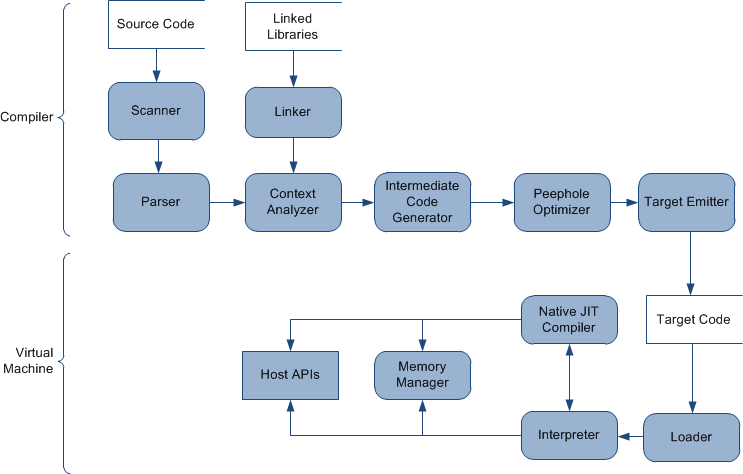
\includegraphics[scale=0.60]{../../images/compiler_data_flow.png}

The following section gives a brief overview of the major
architectural components the comprise the Objeck language compiler and
virtual machine.

\subsection{Compiler}
The language compiler is written in C++ and makes heavy use of the C++
STL for portability across platforms.  As mentioned in the
introduction, the compiler accepts source files and shared libraries
as inputs and produces either executables or shared libraries.  Note,
the compiler has two modes of operation: \texttt{User Mode} compiles
traditional end-user programs, while \texttt{System Mode} compiles
system libraries and processes special system language directives.

\subsubsection{Scanner and Parser}
The scanner component reads source files and parses the text into
tokens.  The scanner works in conjugation with the \emph{LL(k)} parser
by providing \emph{k} lookahead tokens for parsing.  Note, the scanner
can only scan system language directives while in \texttt{System
  Mode}.  The source parser is a recursive-decent parser that
generates an abstract parser tree, which is passed to the Contextual
Analyser for validation.

\subsubsection{Contextual Analyser}
The Contextual Analyser is responsible for ensuring that a source
program is valid.  In addition, the context analyser also creates
relationships between contextually resolved entities (i.e. methods
$\longleftrightarrow$ method calls).  The analyser accepts an abstract
parser tree and shared libraries as input and produces a decorated
parse tree as output.  The decorated parse tree is then passed to the
Intermediate Code Generator for the production of VM instructions.

\subsubsection{Intermediate Code Generator and Optimzier}
The Intermediate Code Generator accpets a decorated parse and produces
a flat list of VM stack instructions.  These instruction lists are
then passed to the Optimizer for basic block optimizations (constant
folding, strength reduction, instruction simplification and method
inlining).

\subsubsection{Target Emitter}
Finally, the improved intermediate code is passed to code emitter
component, which writes it to a file.

\subsection{Virtual Machine}
The language VM is written in C/C++ and was designed to be highly
portable.  The VM makes heavy use of operating system specific APIs
(i.e. WIN32 and POSIX) but does so in an abstracted manner.  The JIT
compiler is targeted to produce machine code for the IA-32 and AMD64
(future) hardware architectures.

\subsubsection{Loader}
The loader component allows the VM to read target code structures such
as classes, methods and VM instructions.  The loader create an
in-memory representation of this information, which is used by the VM
interpreter and JIT compiler.  In addition, the loader processes
command-line parameters that are passed into the VM prior to
execution.

\subsubsection{Interpreter}
The Interpreter executes stack based VM instructions (listed below)
and manages two primary stacks: the execution stack and call stack.
The execution stack is used to manage the data that is needed for VM
calculations.  The call stack is used to manage function/method calls
and the states between those calls.

\subsubsection{JIT Compiler}
The JIT compiler translates stack based VM instruction into processor
specific machine code (i.e. IA-32).  The JIT compiler is evoked by the
interpreter and methods are translated in a separate execution thread.
This process allow methods to be executed concurrently in an
interpreted manner while they are being compiled into machine code.
Note, methods are only converted into machine code once.

\subsubsection{Memory Manager}
The Memory Manager component allows the runtime system to manage the
user allocation/deallocation of heap memory.  The memory mangers
implementes a multi-thread ``mark and sweep'' algorithm.  The marking
stage of the process is multi-thread, such that, each root in scanned
in a separate thread.  The sweeping stage is done in a single thread
since the data structures that are needed to manage the state of the
running program are modified.

\section{Appendix C: VM Instruction Set}
The appendix below lists the types of stack instructions that are
executed by the Objeck VM.  The VM was designed to be portable and
language independent.  Early development versions of the VM included
an inline assembler, which may be re-added in future releases.

\begin{center}
  \begin{tabular}{| l | l | p{6 cm} |}
    \hline
    \multicolumn{3}{|c|}{\textbf{Stack Operators}} \\
    \hline
    \emph{Mnemonic}  &  \emph{Opcode(s)}  &  \emph{Description} \\ \hline \hline
    LOAD\_INT\_LIT & 4-byte integer & pushes integer onto stack  \\ \hline
    LOAD\_FLOAT\_LIT & 8-byte float & pushes float onto stack \\ \hline
    LOAD\_INT\_VAR & variable index & pushes integer onto stack \\ \hline
    LOAD\_FLOAT\_VAR & variable index & pushes float onto stack \\ \hline
    LOAD\_FUNC\_VAR & variable index & pushes float onto stack \\ \hline
    LOAD\_SELF & n/a & pushes self integer on stack \\ \hline
    STOR\_INT\_VAR & variable index & pops integer from stack and saves to index location \\ \hline
    STOR\_FLOAT\_VAR & variable index & pops float from stack and saves to index location \\ \hline
    STOR\_FUNC\_VAR & variable index & pops float from stack and saves to index location \\ \hline
    COPY\_INT\_VAR & variable index & copies an integer from stack and saves to index location \\ \hline
    COPY\_FLOAT\_VAR & variable index & copies a float from stack and saves to index location \\ \hline
    LOAD\_BYTE\_ARY\_ELM & array dimension & pushes byte onto stack; assumes array address was pushed prior \\ \hline
    LOAD\_INT\_ARY\_ELM & array dimension & pushes integer onto stack; assumes array address was pushed prior \\ \hline
    LOAD\_FLOAT\_ARY\_ELM & array dimension & pushes float onto stack; assumes array address was pushed prior \\ \hline
    LOAD\_ARY\_SIZE & n/a & pushes array size as integer onto stack; assumes array address was pushed prior \\ \hline
    STOR\_BYTE\_ARY\_ELM & variable index & stores byte at index location; assumes array address was pushed prior \\ \hline
    STOR\_INT\_ARY\_ELM & variable index & stores integer at index location ; assumes array address was pushed prior \\ \hline
    STOR\_FLOAT\_ARY\_ELM & variable index & stores float at index location; assumes array address was pushed prior \\ \hline
  \end{tabular}

  \vspace{\baselineskip}
  \begin{tabular}{| l | l | p{6 cm} |}
    \hline
    \multicolumn{3}{|c|}{\textbf{Logical Operators}} \\
    \hline
    \emph{Mnemonic}  &  \emph{Opcode(s)}  &  \emph{Description} \\ \hline \hline
    EQL\_INT & n/a & pops top two integer values and pushes result of equal operation \\ \hline
    NEQL\_INT & n/a & pops top two integer values and pushes result of not-equal operation \\ \hline
    LES\_INT & n/a & pops top two integer values and pushes result of less-than operation \\ \hline
    GTR\_INT & n/a & pops top two integer values and pushes result of greater-than operation \\ \hline
    LES\_EQL\_INT & n/a & pops top two integer values and pushes result of less-than-equal operation \\ \hline
    GTR\_EQL\_INT & n/a & pops top two integer values and pushes result of greater-than-equal operation \\ \hline
    EQL\_FLOAT & n/a & pops top two floats values and pushes result of equal operation \\ \hline
    NEQL\_FLOAT & n/a & pops top two floats values and pushes result of not-equal operation \\ \hline
    LES\_FLOAT & n/a & pops top two floats values and pushes result of less-than operation \\ \hline
    GTR\_FLOAT & n/a & pops top two floats values and pushes result of greater-than operation \\ \hline
    LES\_EQL\_FLOAT & n/a & pops top two floats values and pushes result of less-than-equal operation \\ \hline
    GTR\_EQL\_FLOAT & n/a & pops top two floats values and pushes result of greater-than-equal operation \\ \hline
  \end{tabular}

  \vspace{\baselineskip}
  \begin{tabular}{| l | l | p{6 cm} |}
    \hline
    \multicolumn{3}{|c|}{\textbf{Logical Operators}} \\
    \hline
    \emph{Mnemonic}  &  \emph{Opcode(s)}  &  \emph{Description} \\ \hline \hline
    AND\_INT & n/a & pops top two integer values and pushes result of add operation \\ \hline
    OR\_INT & n/a & pops top two integer values and pushes result of or operation \\ \hline
  \end{tabular}

  \vspace{\baselineskip}
  \begin{tabular}{| l | l | p{6 cm} |}
    \hline
    \multicolumn{3}{|c|}{\textbf{Mathematical Operators}} \\
    \hline
    \emph{Mnemonic}  &  \emph{Opcode(s)}  &  \emph{Description} \\ \hline \hline
    ADD\_INT & n/a & pops top two integer values and pushes result of add operation \\ \hline
    SUB\_INT & n/a & pops top two integer values and pushes result of subtract operation \\ \hline
    MUL\_INT & n/a & pops top two integer values and pushes result of multiply operation \\ \hline
    DIV\_INT & n/a & pops top two integer values and pushes result of divide operation \\ \hline
    SHL\_INT & n/a & pops top two floats values and pushes result of shift left operation \\ \hline
    SHR\_INT & n/a & pops top two floats values and pushes result of shift right operation \\ \hline
    MOD\_INT & n/a & pops top two integer values and pushes result of modulus operation \\ \hline
    ADD\_FLOAT & n/a & pops top two floats values and pushes result of greater-than-equal operation \\ \hline
    SUB\_FLOAT & n/a & pops top two floats values and pushes result of subtract operation \\ \hline
    MUL\_FLOAT & n/a & pops top two floats values and pushes result of multiply operation \\ \hline
    DIV\_FLOAT & n/a & pops top two floats values and pushes result of divide operation \\ \hline
    I2F & n/a & pop top integer and pushes result of float cast \\ \hline
    F2I & n/a & pop top float and pushes result of integer cast \\ \hline
  \end{tabular}

  \vspace{\baselineskip}
  \begin{tabular}{| l | p{4 cm} | p{6 cm} |}
    \hline
    \multicolumn{3}{|c|}{\textbf{Methods}} \\
    \hline
    \emph{Mnemonic}  &  \emph{Opcode(s)}  &  \emph{Description} \\ \hline \hline
    SWAP\_INT & n/a & swaps the top two integer values on the stack \\ \hline
    POP\_INT & n/a & control pop of an integer from the stack \\ \hline
    POP\_FLOAT & n/a & control pop of a float from the stack \\ \hline
    RTRN & n/a & exits existing method returning control to callee \\ \hline
    MTHD\_CALL & integer values for class id and method id & synchronous call to given method releasing control \\ \hline
    DYN\_MTHD\_CALL & pops integer values for class id and method id & dynamic synchronous call to given method releasing control \\ \hline
    ASYNC\_MTHD\_CALL & integer values for class id and method id; pushes new thread id & asynchronous call to given method \\ \hline
    ASYNC\_JOIN & thread id & waits for identified thread to end execution \\ \hline
    LBL & label id & identifies a jump label \\ \hline
\end{tabular}

\vspace{\baselineskip}
  \begin{tabular}{| l | p{4 cm} | p{6 cm} |}
    \hline
    \multicolumn{3}{|c|}{\textbf{Objects and Memory Operations}} \\
    \hline
    \emph{Mnemonic}  &  \emph{Opcode(s)}  &  \emph{Description} \\ \hline \hline
    JMP & label id and conditional context (1=true, 0=unconditional, -1=false) & jump to label id \\ \hline
    NEW\_BYTE\_ARY & array dimension & pushes address of new byte array \\ \hline
    NEW\_INT\_ARY & array dimension & pushes address of new integer array \\ \hline
    NEW\_FLOAT\_ARY & array dimension & pushes address of new float array \\ \hline
    NEW\_OBJ\_INST & integer value for class id & pushes address of new class instance \\ \hline
    OBJ\_TYPE\_OF & integer value of ``check'' class & performs runtime object instance check \\ \hline
    OBJ\_INST\_CAST & integer values for ``from'' class and ``to''
    class & performs runtime class cast check (note: only required for
    up casting) \\ \hline
    CPY\_BYTE\_ARY & destination of source array, offset of destination array,
    address of source array, offset of source array, number of
    & copies elements from one array to another \\ \hline
    CPY\_INT\_ARY & destination of source array, offset of destination array,
    address of source array, offset of source array, number of
    & copies elements from one array to another \\ \hline
    CPY\_FLOAT\_ARY & destination of source array, offset of destination array,
    address of source array, offset of source array, number of
    & copies elements from one array to another \\ \hline
  \end{tabular}

  \vspace{\baselineskip}
  \begin{tabular}{| l | p{4 cm} | p{6 cm} |}
    \hline
    \multicolumn{3}{|c|}{\textbf{Traps and Threads}} \\
    \hline
    \emph{Mnemonic}  &  \emph{Opcode(s)}  &  \emph{Description} \\ \hline \hline
    THREAD\_CREATE & n/a & creates an new thread instance (calculation stack and  stack pointer) \\ \hline
    THREAD\_WAIT & n/a & waits for worker threads to stop execution \\ \hline
    CRITICAL\_START & n/a & creates a mutex such that only one thread can execute in a given section \\ \hline
    CRITICAL\_END & n/a & releases a system mutex \\ \hline
    TRAP & integer value for trap id & calls runtime subroutine releasing control \\ \hline
    TRAP\_RTRN & integer value for trap id and number of arguments &
    calls runtime subroutine releasing control and then processes an integer return value \\ \hline
    LIB\_NEW\_OBJ\_INST & n/a & symbolic library link for a new object instance  \\ \hline
    LIB\_MTHD\_CALL & n/a & symbolic library link for a method call  \\ \hline
    LIB\_OBJ\_INST\_CAST & n/a & symbolic library link for an object cast  \\ \hline
  \end{tabular}
\end{center}

\end{document}
